\section{Exercícios}

\begin{exercise}
    Na Definição~\ref{def:seno-cosseno-triangulo-retangulo}, definimos seno e cosseno de um ângulo no
triângulo retângulo. Como você definiria, com os lados de um
triângulo retângulo, as demais relações trigonométricas da Definição
\ref{def:outras-funcoes-trigonometricas}?
\end{exercise}

\begin{exercise}
  Encontre os valores do domínio da função $\sen$ tais que ela seja igual a $-1$, $0$ e $1$ (não simultaneamente). 
  Repita o processo para as funções $\cos$, $\tan$, $\sec$, $\csc$ e $\cot$.
\end{exercise}

\begin{exercise}
    A figura abaixo representa o gráfico da função $f_1 : \R \to
\R$, $f_1(x) = x \cdot \sen x$, traçado no intervalo $\bracket{-20 \pi,
20 \pi}$, juntamente com as retas $y=x$ e $y=-x$.
\begin{center}
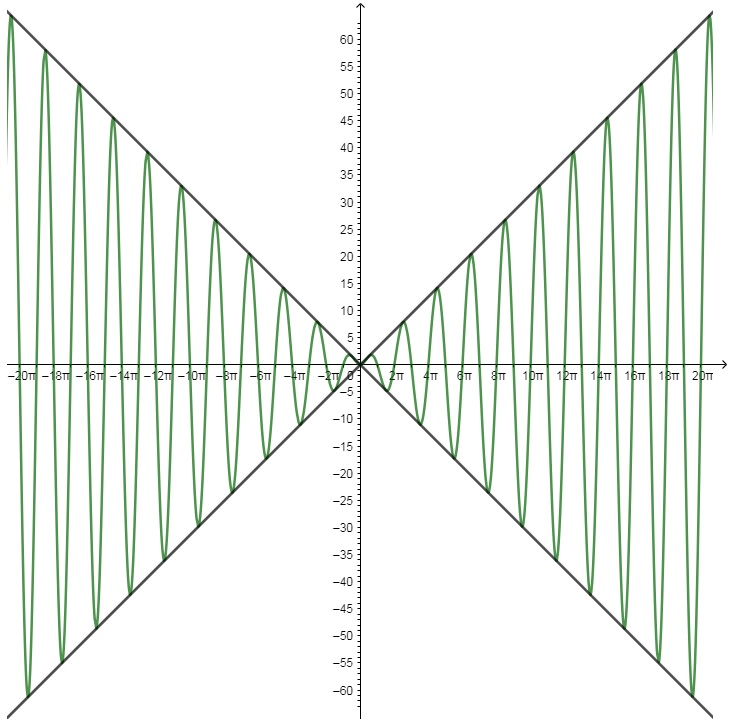
\includegraphics[scale=0.35]{\imgdirfromsection/grafxsenx.jpg}
\end{center}
\begin{enumerate}[a)]
  \item Explique por que o gráfico de $f_1$ fica limitado entre
  essas retas e indique todos os pontos em que o gráfico toca as retas;
  \item Considere a seguinte afirmação: \emph{Os máximos e
  mínimos locais da função $f_1$ ocorrem nos mesmos valores
  de $x$ que os da função seno.} Esta afirmação é verdadeira?
  \item Como você espera visualizar o gráfico da função $f_2: \R \to
  \R$, definida por $f_2(x) = x^2 \cdot \sen x$?
\end{enumerate}
\end{exercise}

\begin{exercise}
    Na figura abaixo, temos um círculo trigonométrico e os segmentos $AD$ e $OD$ representam,
respectivamente, $\tan x$ e $\sec x$.
\begin{center}
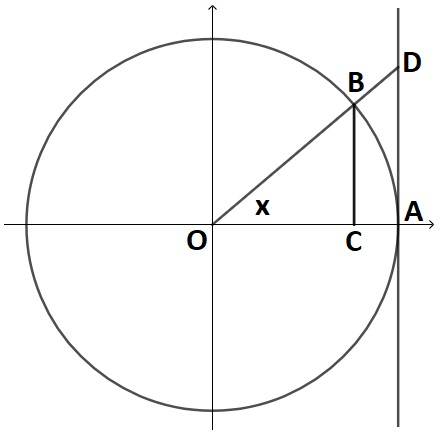
\includegraphics[scale=0.5]{\imgdirfromsection/circtansec.jpg}
\end{center}
\begin{enumerate}[a)]
  \item Justifique a afirmação acima;
  \item Qual a interpretação dos sinais de $\tan x$ e $\sec x$ na
  figura?
  \item Faça uma figura análoga para representar $\cot x$ e $\csc
  x$, justificando a construção.
\end{enumerate}
\end{exercise}

\begin{exercise}
    Encontre as três menores soluções positivas da equação $$\cos
\paren{3x - \frac {\pi} 4} = 0.$$
\end{exercise}

\begin{exercise}
  Sem utilizar as fórmulas de seno e cosseno da soma de dois arcos,
  mostre que, para todo $t\in\reals$, vale \[\cos\prn{\frac \pi 2-t}=\sen t\]
\end{exercise}

\begin{exercise}
  Considere um triângulo retângulo tal que seu perímetro é igual a $\dfrac{\raiz 6 + 2}{2}$ e sua hipotenusa mede $1$. Calcule a medida do menor de seus ângulos.
\end{exercise}

\begin{exercise}
    Mostre que o perímetro do pentágono regular inscrito em um
círculo unitário é dado por $10\sen \frac {\pi} 5$.
\end{exercise}

\begin{exercise}
    Considere a função $f: \R \to \R$ definida por $f(x) = \sen
\paren{ax}+\sen \paren{bx}$, em que $a$ e $b$ são constantes reais.
\begin{enumerate}[a)]
  \item Mostre que, se $a$ e $b$ são racionais, então $f$ é
  periódica;\\
  \emph{Dica:} Mostre que o período de $\sen \paren{ax}$ é $\frac
  {2\pi} a$.
  \item A recíproca da afirmação do item anterior é verdadeira?
  Justifique sua resposta.
\end{enumerate}
\end{exercise}

\begin{exercise}
    Prove as identidades abaixo, válidas para todo $x$ onde as
expressões estão definidas:
\begin{enumerate}[a)]
  \item $\dfrac{1-\tan^2 x}{1+\tan^2 x} = 1 - 2\sen^2 x$;
  \item $\dfrac{\cos x - \sen x}{\cos x + \sen x} = \dfrac{1 - \tan x}{1+\tan
  x}$;
  \item $\dfrac{\sen x}{\csc x - \cot x} = 1+ \cos x$;
  \item $\cos^2 x = \dfrac {1+\cos \paren{2x}} 2$;
  \item $\sen^2 x = \dfrac {1-\cos \paren{2x}} 2$;
  \item $\sen(mx)\cdot\cos(nx)=\dfrac{\sen[(m-n)x]-\sen[(m+n)x]}{2}$;
  \item $\sen(mx)\cdot\sen(nx)=\dfrac{\cos[(m-n)x]-\cos[(m+n)x]}{2}$;
  \item $\dfrac{1-\tan^2 x}{1+\tan^2 x} = \cos^2 x - \sen^2 x = \cos \paren{2x}$;
  \item $\dfrac{2\tan x}{1+\tan^2 x} = 2\sen x \cos x= \sen\paren{2x}$.
\end{enumerate}
\end{exercise}

\begin{exercise}
    Use as fórmulas de seno e cosseno da soma para determinar os
senos e cossenos dos seguintes ângulos (medidos em radianos): $\frac
{\pi} 8$, $\frac{\pi} {12}$, $\frac {3\pi} 8$ e $\frac{5\pi}{12}$.
\end{exercise}

\begin{exercise}
  Considere dois ângulos $\alpha$ e $\beta$, tais que $0 < \alpha < \dfrac \pi 2$ e $0 < \beta < \dfrac \pi 2$. Na figura abaixo temos um círculo trigonométrico, onde são marcados os pontos $A$, $B$, $C$ e $D$ de tal sorte que $\alpha = \widehat{AOB}$ e $\beta = \widehat{BOC} = \widehat{AOD}$.
  \begin{center}
    \importtikz{exercicio-cos_da_soma}
    \label{fig:cos-da-soma}
  \end{center}
  \begin{enumerate}[a)]
    \item Utilizando os conceitos de trigonometria, escreva as coordenadas dos pontos $A$, $B$, $C$ e $D$;
    \item Determine $\overline{AC}$ (medida do comprimento do segmento $AC$) em função das coordenadas de $A$ e $C$;
    \item Determine $\overline{BD}$ em função das coordenadas de $B$ e $D$;
    \item Sabendo que $\overline{AC} = \overline{BD}$, use os itens anteriores para mostrar a fórmula para $\cos (\alpha + \beta)$.
    \end{enumerate}
\end{exercise}

\begin{exercise}
    Obtenha fórmulas para: 
    \begin{enumerate}[a)]
      \item $\tan\paren{\alpha + \beta}$ em função de $\tan \alpha$ e $\tan \beta$;
      \item $\tan\paren{\alpha - \beta}$ em função de $\tan \alpha$ e $\tan \beta$;
      \item $\tan\paren{2 \alpha}$ em função de $\tan \alpha$;
      \item $\sec \paren{\alpha + \beta}$ em função de $\sec \alpha$, $\sec \beta$, $\tan \alpha$ e $\tan \beta$.
    \end{enumerate}
\end{exercise}

\begin{exercise}
  Pedro afirma que, em competições de tiro, acertar um alvo na diagonal é mais difícil do que acertar um alvo que está à frente por conta que o ângulo de visão do alvo na diagonal é menor. A figura \ref{fig:angulos-de-visao} (fora de escala) simula uma situação em uma competição de tiros, onde Pedro está no ponto P a 25m de distância do alvo à frente, cada alvo tem 0,5m de diâmetro e distam 4,75m um do outro.
        \begin{figure}[H]
          \centering 
          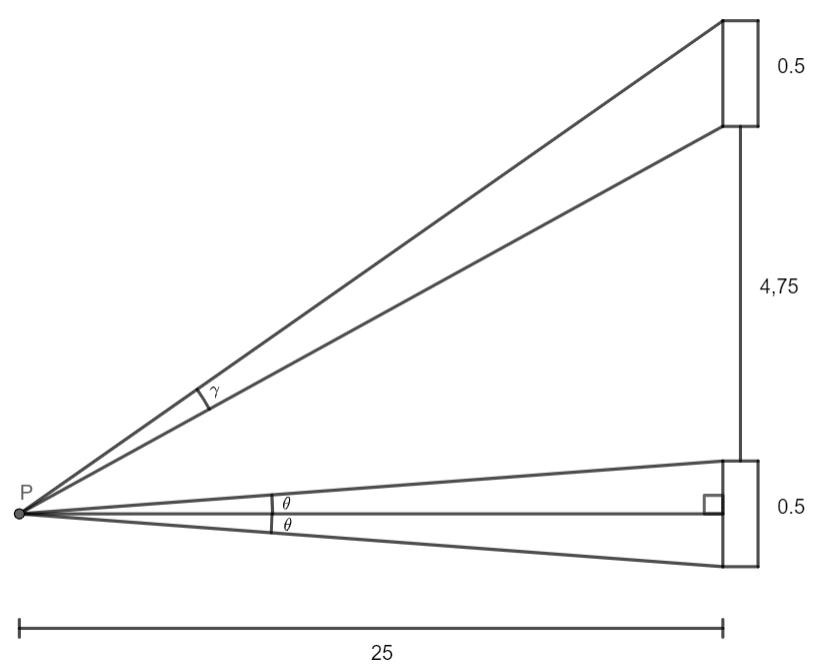
\includegraphics[width=10cm]{\imgdirfromsection/exercicio-angulos-de-visao.png} 
          \caption{Ângulos de visão dos alvos}
          \label{fig:angulos-de-visao}
        \end{figure}
        Com a notação da figura, mostre que o ângulo de visão do alvo na diagonal é menor que o ângulo de visão do alvo à frente, ou seja, $\gamma < 2\theta$. Para tanto, use o conceito de tangente no triângulo retângulo, o fato de tangente ser uma função crescente. É permitido o uso de uma calculadora para contas básicas de soma, multiplicação e divisão.
\end{exercise}
